\documentclass{article}

\usepackage{arxiv}

\usepackage[utf8]{inputenc} % allow utf-8 input
\usepackage[T1]{fontenc}    % use 8-bit T1 fonts
\usepackage{lmodern}        % https://github.com/rstudio/rticles/issues/343
\usepackage{hyperref}       % hyperlinks
\usepackage{url}            % simple URL typesetting
\usepackage{booktabs}       % professional-quality tables
\usepackage{amsfonts}       % blackboard math symbols
\usepackage{nicefrac}       % compact symbols for 1/2, etc.
\usepackage{microtype}      % microtypography
\usepackage{graphicx}

\title{Explaining time series downsampling through visualisation}

\author{
    Morgan Frodsham
   \\
    School of Computing \\
    Newcastle University \\
  Newcastle upon Tyne, UK \\
  \texttt{\href{mailto:M.C.M.Frodsham2@newcastle.ac.uk}{\nolinkurl{M.C.M.Frodsham2@newcastle.ac.uk}}} \\
   \And
    Matthew Forshaw
   \\
    School of Computing \\
    Newcastle University \\
  Newcastle upon Tyne, UK \\
  \texttt{\href{mailto:matthew.forshaw@newcastle.ac.uk}{\nolinkurl{matthew.forshaw@newcastle.ac.uk}}} \\
  }

% Pandoc syntax highlighting
\usepackage{color}
\usepackage{fancyvrb}
\newcommand{\VerbBar}{|}
\newcommand{\VERB}{\Verb[commandchars=\\\{\}]}
\DefineVerbatimEnvironment{Highlighting}{Verbatim}{commandchars=\\\{\}}
% Add ',fontsize=\small' for more characters per line
\usepackage{framed}
\definecolor{shadecolor}{RGB}{248,248,248}
\newenvironment{Shaded}{\begin{snugshade}}{\end{snugshade}}
\newcommand{\AlertTok}[1]{\textcolor[rgb]{0.94,0.16,0.16}{#1}}
\newcommand{\AnnotationTok}[1]{\textcolor[rgb]{0.56,0.35,0.01}{\textbf{\textit{#1}}}}
\newcommand{\AttributeTok}[1]{\textcolor[rgb]{0.77,0.63,0.00}{#1}}
\newcommand{\BaseNTok}[1]{\textcolor[rgb]{0.00,0.00,0.81}{#1}}
\newcommand{\BuiltInTok}[1]{#1}
\newcommand{\CharTok}[1]{\textcolor[rgb]{0.31,0.60,0.02}{#1}}
\newcommand{\CommentTok}[1]{\textcolor[rgb]{0.56,0.35,0.01}{\textit{#1}}}
\newcommand{\CommentVarTok}[1]{\textcolor[rgb]{0.56,0.35,0.01}{\textbf{\textit{#1}}}}
\newcommand{\ConstantTok}[1]{\textcolor[rgb]{0.00,0.00,0.00}{#1}}
\newcommand{\ControlFlowTok}[1]{\textcolor[rgb]{0.13,0.29,0.53}{\textbf{#1}}}
\newcommand{\DataTypeTok}[1]{\textcolor[rgb]{0.13,0.29,0.53}{#1}}
\newcommand{\DecValTok}[1]{\textcolor[rgb]{0.00,0.00,0.81}{#1}}
\newcommand{\DocumentationTok}[1]{\textcolor[rgb]{0.56,0.35,0.01}{\textbf{\textit{#1}}}}
\newcommand{\ErrorTok}[1]{\textcolor[rgb]{0.64,0.00,0.00}{\textbf{#1}}}
\newcommand{\ExtensionTok}[1]{#1}
\newcommand{\FloatTok}[1]{\textcolor[rgb]{0.00,0.00,0.81}{#1}}
\newcommand{\FunctionTok}[1]{\textcolor[rgb]{0.00,0.00,0.00}{#1}}
\newcommand{\ImportTok}[1]{#1}
\newcommand{\InformationTok}[1]{\textcolor[rgb]{0.56,0.35,0.01}{\textbf{\textit{#1}}}}
\newcommand{\KeywordTok}[1]{\textcolor[rgb]{0.13,0.29,0.53}{\textbf{#1}}}
\newcommand{\NormalTok}[1]{#1}
\newcommand{\OperatorTok}[1]{\textcolor[rgb]{0.81,0.36,0.00}{\textbf{#1}}}
\newcommand{\OtherTok}[1]{\textcolor[rgb]{0.56,0.35,0.01}{#1}}
\newcommand{\PreprocessorTok}[1]{\textcolor[rgb]{0.56,0.35,0.01}{\textit{#1}}}
\newcommand{\RegionMarkerTok}[1]{#1}
\newcommand{\SpecialCharTok}[1]{\textcolor[rgb]{0.00,0.00,0.00}{#1}}
\newcommand{\SpecialStringTok}[1]{\textcolor[rgb]{0.31,0.60,0.02}{#1}}
\newcommand{\StringTok}[1]{\textcolor[rgb]{0.31,0.60,0.02}{#1}}
\newcommand{\VariableTok}[1]{\textcolor[rgb]{0.00,0.00,0.00}{#1}}
\newcommand{\VerbatimStringTok}[1]{\textcolor[rgb]{0.31,0.60,0.02}{#1}}
\newcommand{\WarningTok}[1]{\textcolor[rgb]{0.56,0.35,0.01}{\textbf{\textit{#1}}}}

% tightlist command for lists without linebreak
\providecommand{\tightlist}{%
  \setlength{\itemsep}{0pt}\setlength{\parskip}{0pt}}

% From pandoc table feature
\usepackage{longtable,booktabs,array}
\usepackage{calc} % for calculating minipage widths
% Correct order of tables after \paragraph or \subparagraph
\usepackage{etoolbox}
\makeatletter
\patchcmd\longtable{\par}{\if@noskipsec\mbox{}\fi\par}{}{}
\makeatother
% Allow footnotes in longtable head/foot
\IfFileExists{footnotehyper.sty}{\usepackage{footnotehyper}}{\usepackage{footnote}}
\makesavenoteenv{longtable}

% Pandoc citation processing
\newlength{\cslhangindent}
\setlength{\cslhangindent}{1.5em}
\newlength{\csllabelwidth}
\setlength{\csllabelwidth}{3em}
\newlength{\cslentryspacingunit} % times entry-spacing
\setlength{\cslentryspacingunit}{\parskip}
% for Pandoc 2.8 to 2.10.1
\newenvironment{cslreferences}%
  {}%
  {\par}
% For Pandoc 2.11+
\newenvironment{CSLReferences}[2] % #1 hanging-ident, #2 entry spacing
 {% don't indent paragraphs
  \setlength{\parindent}{0pt}
  % turn on hanging indent if param 1 is 1
  \ifodd #1
  \let\oldpar\par
  \def\par{\hangindent=\cslhangindent\oldpar}
  \fi
  % set entry spacing
  \setlength{\parskip}{#2\cslentryspacingunit}
 }%
 {}
\usepackage{calc}
\newcommand{\CSLBlock}[1]{#1\hfill\break}
\newcommand{\CSLLeftMargin}[1]{\parbox[t]{\csllabelwidth}{#1}}
\newcommand{\CSLRightInline}[1]{\parbox[t]{\linewidth - \csllabelwidth}{#1}\break}
\newcommand{\CSLIndent}[1]{\hspace{\cslhangindent}#1}

\begin{document}
\maketitle


\begin{abstract}
Enter the text of your abstract here.
\end{abstract}

\keywords{
    blah
   \and
    blee
   \and
    bloo
   \and
    these are optional and can be removed
  }

\twocolumn

\hypertarget{introduction}{%
\section{INTRODUCTION}\label{introduction}}

The UK Government is committed to making data-driven decisions that
engender public trust
\protect\hyperlink{ref-data2017}{{[}1{]}}--\protect\hyperlink{ref-data2022}{{[}4{]}}.
Data-driven decisions are considered to be ``more well-informed''
\protect\hyperlink{ref-data2017}{{[}1{]}}, effective
\protect\hyperlink{ref-data2022}{{[}4{]}}, consistent
\protect\hyperlink{ref-data2021}{{[}3{]}}, and better ``at scale''
\protect\hyperlink{ref-data2020}{{[}2{]}}. Despite this, there is a lack
of trust in government use of data
\protect\hyperlink{ref-trust}{{[}5{]}}. This suggests that public trust
in data-driven decisions goes beyond how the ``data complies with legal,
regulatory and ethical obligations''
\protect\hyperlink{ref-data2021}{{[}3{]}}. Transparency is needed for
the UK public to have ``confidence and trust in how data, including
personal data, is used'' \protect\hyperlink{ref-data2020}{{[}2{]}},
\protect\hyperlink{ref-trust}{{[}5{]}}.

To make data-driven decisions, government decision-makers also need to
trust how the data used (cite user research here). This means trusting
which data points are selected, how this data collected and stored, and
the capability of data practitioners to understand the quality, insights
and limitations of it. At every stage of the data processing pipeline,
data practitioners have the opportunity to communicate the impact of the
assumptions and choices they are making to support decision-makers in
trusting the data informing their decisions.

Time series data is used across the UK Government
\protect\hyperlink{ref-pathway}{{[}6{]}} to inform decision-makers
across various domains \protect\hyperlink{ref-onstool}{{[}7{]}}. It is
also widely generated and used by industry and research
\protect\hyperlink{ref-TVStore}{{[}8{]}}. The volume of time series data
is continuously increasingly \protect\hyperlink{ref-datapoint}{{[}9{]}},
posing significant challenges for handling and visualising this popular
data type \protect\hyperlink{ref-TVStore}{{[}8{]}}. Data practitioners
must utilise methods that reduce data volumes to align with limitations
like processing time, computing costs, storage capabilities, and
sustainability ambitions \protect\hyperlink{ref-TVStore}{{[}8{]}},
\protect\hyperlink{ref-Sveinn}{{[}10{]}},
\protect\hyperlink{ref-Shift}{{[}11{]}}.

Downsampling is an established technique
\protect\hyperlink{ref-downsampling}{{[}12{]}},
\protect\hyperlink{ref-sampling}{{[}13{]}} that involves selecting a
representative subset of the time series data to preserve its shape
while reducing the number of data points
\protect\hyperlink{ref-datapoint}{{[}9{]}},
\protect\hyperlink{ref-MinMaxLTTB}{{[}14{]}}. This is a vital part of
making voluminous time series understandable for human observation
\protect\hyperlink{ref-Sveinn}{{[}10{]}} and an essential step in many
time series database solutions
\protect\hyperlink{ref-datapoint}{{[}9{]}}. However, little attention
has been devoted to how downsampling impacts decision-makers trust in
the data.

Despite widespread use, how to communicate the impact of downsampling
algorithms on time series data remains understudied
\protect\hyperlink{ref-datapoint}{{[}9{]}},
\protect\hyperlink{ref-Sveinn}{{[}10{]}}. Downsampling expands the
boundaries of risk for decision-makers as data practitioners may not
realise the significance of the data being discarded. Such choices
throughout the data pipeline may have disproportionately larger
consequences later as their ramifications for future decisions are not
fully understood by all. It is important, therefore, that data
practitioners are able to communicate the impact of choices made
throughout the data pipeline.

To address these challenges, this work proposes a visualisation
methodology for understanding and communicating the impact of
downsampling algorithms on time series data. Section \emph{II}
contextualises the impact of this work for data practitioners and
decision-makers by sharing insights from user research. Section
\emph{III} provides an overview of previous related work to help assess
the contributions of this work. Section \emph{IV} presents how R
packages \texttt{imputeTS} \protect\hyperlink{ref-imputeTS_R}{{[}15{]}}
and \texttt{Rcatch22}
\protect\hyperlink{ref-Rcatch22}{\textbf{Rcatch22?}} are combined to
identify the time series features that are most sensitive to
downsampling. Section \emph{V} outlines how this approach allows data
practitioners to communicate which downsampling algorithms and
parameters are most appropriate for particular use cases. Section
\emph{VI} shares the potential impact of this work and the opportunities
for further work to improve decision-makers' trust in data.

\hypertarget{motivation}{%
\section{MOTIVATION}\label{motivation}}

\label{sec:headings}

\hypertarget{related-work}{%
\section{RELATED WORK}\label{related-work}}

\label{sec:headings}

\emph{A. Downsampling applications and processes}

Data-driven decision-making necessitates that time series data is kept
for future analysis. Technological innovation has generated
unprecedented amount of time series data, which continues to grow
\protect\hyperlink{ref-data2020}{{[}2{]}},
\protect\hyperlink{ref-storage}{{[}16{]}},
\protect\hyperlink{ref-CatchUp}{{[}17{]}},
\protect\hyperlink{ref-TVstore}{\textbf{TVstore?}}. For example, climate
simulations that inform recommendations for decision-makers generate
tens of terabytes per second. Downsampling plays an important role in
addressing how this voluminous data is processed, stored
\protect\hyperlink{ref-TVstore}{\textbf{TVstore?}} and visualised
\protect\hyperlink{ref-Sveinn}{{[}10{]}},
\protect\hyperlink{ref-dashql}{{[}18{]}}.

Data practitioners have made recent advances in the performance of value
preserving downsampling algorithms
\protect\hyperlink{ref-downsampling}{{[}12{]}},
\protect\hyperlink{ref-MinMaxLTTB}{{[}14{]}},
\protect\hyperlink{ref-dashql}{{[}18{]}}--\protect\hyperlink{ref-MinMaxOrdered}{{[}20{]}},
\protect\hyperlink{ref-samping}{\textbf{samping?}}. Examples of these
advances are set out in the table below:

insert table \protect\hyperlink{ref-datapoint}{{[}9{]}} - EveryNth, also
known as sampling or decimation, selects \emph{n\textsuperscript{th}}
datapoint \protect\hyperlink{ref-EveryNth}{{[}19{]}} - percentage change
- MinMax preserves the minimum and maximum of every data bucket
\protect\hyperlink{ref-MinMaxLTTB}{{[}14{]}} - OM\textsuperscript{3}
maintains minimum and maximum values at every time interval that is used
to rasterize a pixel column in the display window
\protect\hyperlink{ref-MinMaxOrdered}{{[}20{]}} - M4 combines EveryNth
and MinMax, selecting the first and last values of each data bucket as
well as its minimum and maximum
\protect\hyperlink{ref-dashql}{{[}18{]}},
\protect\hyperlink{ref-M4}{{[}21{]}} - Largest-TriangleOne-Bucket (LTOB)
- Largest Triangle Three Buckets LTTB selects the data point that forms
the largest triangular surface between the previously selected data
point and the next data bucket's average value
\protect\hyperlink{ref-MinMaxLTTB}{{[}14{]}} - MinMaxLTTB preselects
data using MinMax before applying LTTB on the selected datapoints
\protect\hyperlink{ref-MinLaxLTTB}{\textbf{MinLaxLTTB?}}

\emph{B. Time series visualisation}

\emph{C. Trust in Data}

\onecolumn

You can use directly LaTeX command or Markdown text.

LaTeX command can be used to reference other section. See Section
\ref{sec:headings}. However, you can also use \textbf{bookdown}
extensions mechanism for this.

\hypertarget{headings-second-level}{%
\subsection{Headings: second level}\label{headings-second-level}}

You can use equation in blocks

\[
\xi _{ij}(t)=P(x_{t}=i,x_{t+1}=j|y,v,w;\theta)= {\frac {\alpha _{i}(t)a^{w_t}_{ij}\beta _{j}(t+1)b^{v_{t+1}}_{j}(y_{t+1})}{\sum _{i=1}^{N} \sum _{j=1}^{N} \alpha _{i}(t)a^{w_t}_{ij}\beta _{j}(t+1)b^{v_{t+1}}_{j}(y_{t+1})}}
\]

But also inline i.e \(z=x+y\)

\hypertarget{headings-third-level}{%
\subsubsection{Headings: third level}\label{headings-third-level}}

Another paragraph.

\hypertarget{methodology}{%
\section{METHODOLOGY}\label{methodology}}

\label{sec:headings}

\hypertarget{imputets}{%
\subsection{ImputeTS}\label{imputets}}

\hypertarget{rcatch22}{%
\subsection{Rcatch22}\label{rcatch22}}

\hypertarget{downsamplng-impat}{%
\subsection{Downsamplng Impat}\label{downsamplng-impat}}

\hypertarget{user-research}{%
\subsection{User Research}\label{user-research}}

\hypertarget{results-and-evaluation}{%
\section{RESULTS AND EVALUATION}\label{results-and-evaluation}}

\label{sec:headings}

\hypertarget{future-work}{%
\section{FUTURE WORK}\label{future-work}}

\label{sec:headings}

\hypertarget{conclusion}{%
\section{CONCLUSION}\label{conclusion}}

\label{sec:headings}

\hypertarget{references}{%
\section{REFERENCES}\label{references}}

\label{sec:headings}

\hypertarget{examples-of-citations-figures-tables-references}{%
\section{Examples of citations, figures, tables,
references}\label{examples-of-citations-figures-tables-references}}

\label{sec:others}

You can insert references. Here is some text
\protect\hyperlink{ref-kour2014real}{\textbf{kour2014real?}},
\protect\hyperlink{ref-kour2014fast}{\textbf{kour2014fast?}} and see
\protect\hyperlink{ref-hadash2018estimate}{\textbf{hadash2018estimate?}}.

The documentation for \verb+natbib+ may be found at

You can use custom blocks with LaTeX support from \textbf{rmarkdown} to
create environment.

\begin{center}
\url{http://mirrors.ctan.org/macros/latex/contrib/natbib/natnotes.pdf\%7D}

\end{center}

Of note is the command \verb+\citet+, which produces citations
appropriate for use in inline text.

You can insert LaTeX environment directly too.

\begin{verbatim}
   \citet{hasselmo} investigated\dots
\end{verbatim}

produces

\begin{quote}
  Hasselmo, et al.\ (1995) investigated\dots
\end{quote}

\begin{center}
  \url{https://www.ctan.org/pkg/booktabs}
\end{center}

\hypertarget{figures}{%
\subsection{Figures}\label{figures}}

You can insert figure using LaTeX directly.

See Figure \ref{fig:fig1}. Here is how you add footnotes. {[}\^{}Sample
of the first footnote.{]}

\begin{figure}
  \centering
  \fbox{\rule[-.5cm]{4cm}{4cm} \rule[-.5cm]{4cm}{0cm}}
  \caption{Sample figure caption.}
  \label{fig:fig1}
\end{figure}

But you can also do that using R.

\begin{Shaded}
\begin{Highlighting}[]
\FunctionTok{plot}\NormalTok{(mtcars}\SpecialCharTok{$}\NormalTok{mpg)}
\end{Highlighting}
\end{Shaded}

\begin{figure}
\centering
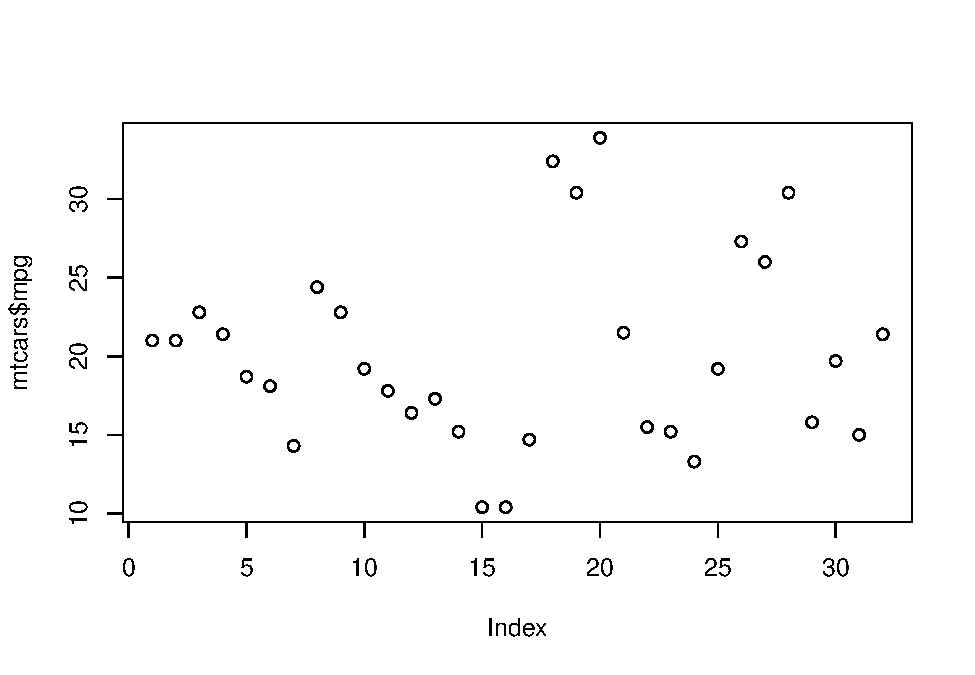
\includegraphics{210431461_CSC8639_Dissertation_files/figure-latex/fig2-1.pdf}
\caption{Another sample figure}
\end{figure}

You can use \textbf{bookdown} to allow references for Tables and
Figures.

\hypertarget{tables}{%
\subsection{Tables}\label{tables}}

Below we can see how to use tables.

See awesome Table\textasciitilde{}\ref{tab:table} which is written
directly in LaTeX in source Rmd file.

\begin{table}
 \caption{Sample table title}
  \centering
  \begin{tabular}{lll}
    \toprule
    \multicolumn{2}{c}{Part}                   \\
    \cmidrule(r){1-2}
    Name     & Description     & Size ($\mu$m) \\
    \midrule
    Dendrite & Input terminal  & $\sim$100     \\
    Axon     & Output terminal & $\sim$10      \\
    Soma     & Cell body       & up to $10^6$  \\
    \bottomrule
  \end{tabular}
  \label{tab:table}
\end{table}

You can also use R code for that.

\begin{Shaded}
\begin{Highlighting}[]
\NormalTok{knitr}\SpecialCharTok{::}\FunctionTok{kable}\NormalTok{(}\FunctionTok{head}\NormalTok{(mtcars), }\AttributeTok{caption =} \StringTok{"Head of mtcars table"}\NormalTok{)}
\end{Highlighting}
\end{Shaded}

\begin{longtable}[]{@{}lrrrrrrrrrrr@{}}
\caption{Head of mtcars table}\tabularnewline
\toprule
& mpg & cyl & disp & hp & drat & wt & qsec & vs & am & gear & carb \\
\midrule
\endfirsthead
\toprule
& mpg & cyl & disp & hp & drat & wt & qsec & vs & am & gear & carb \\
\midrule
\endhead
Mazda RX4 & 21.0 & 6 & 160 & 110 & 3.90 & 2.620 & 16.46 & 0 & 1 & 4 &
4 \\
Mazda RX4 Wag & 21.0 & 6 & 160 & 110 & 3.90 & 2.875 & 17.02 & 0 & 1 & 4
& 4 \\
Datsun 710 & 22.8 & 4 & 108 & 93 & 3.85 & 2.320 & 18.61 & 1 & 1 & 4 &
1 \\
Hornet 4 Drive & 21.4 & 6 & 258 & 110 & 3.08 & 3.215 & 19.44 & 1 & 0 & 3
& 1 \\
Hornet Sportabout & 18.7 & 8 & 360 & 175 & 3.15 & 3.440 & 17.02 & 0 & 0
& 3 & 2 \\
Valiant & 18.1 & 6 & 225 & 105 & 2.76 & 3.460 & 20.22 & 1 & 0 & 3 & 1 \\
\bottomrule
\end{longtable}

\hypertarget{lists}{%
\subsection{Lists}\label{lists}}

\begin{itemize}
\tightlist
\item
  Item 1
\item
  Item 2
\item
  Item 3
\end{itemize}

\hypertarget{refs}{}
\begin{CSLReferences}{0}{0}
\leavevmode\vadjust pre{\hypertarget{ref-data2017}{}}%
\CSLLeftMargin{{[}1{]} }
\CSLRightInline{Cabinet Office and Government Digital Service,
{``Government transformation strategy: Better use of data.''} HM
Government;
\url{https://www.gov.uk/government/publications/government-transformation-strategy-2017-to-2020/government-transformation-strategy-better-use-of-data},
2017.}

\leavevmode\vadjust pre{\hypertarget{ref-data2020}{}}%
\CSLLeftMargin{{[}2{]} }
\CSLRightInline{Department for Digital, Culture, Media \& Sport and
Department for Science, Innovation \& Technology, {``National data
strategy.''} HM Government;
\url{https://www.gov.uk/government/publications/uk-national-data-strategy/national-data-strategy},
2020.}

\leavevmode\vadjust pre{\hypertarget{ref-data2021}{}}%
\CSLLeftMargin{{[}3{]} }
\CSLRightInline{M. of Defence, {``Data strategy for defence,''}
\emph{GOV.UK}. HM Government;
\url{https://www.gov.uk/government/publications/data-strategy-for-defence/data-strategy-for-defence},
2021.}

\leavevmode\vadjust pre{\hypertarget{ref-data2022}{}}%
\CSLLeftMargin{{[}4{]} }
\CSLRightInline{Central Digital \& Data Office, {``Transforming for a
digital future: 2022 to 2025 roadmap for digital and data.''} HM
Government;
\url{https://www.gov.uk/government/publications/roadmap-for-digital-and-data-2022-to-2025/transforming-for-a-digital-future-2022-to-2025-roadmap-for-digital-and-data},
2022.}

\leavevmode\vadjust pre{\hypertarget{ref-trust}{}}%
\CSLLeftMargin{{[}5{]} }
\CSLRightInline{Centre for Data Ethics \& Innovation, {``Addressing
trust in public sector data use.''}
\url{https://www.gov.uk/government/publications/cdei-publishes-its-first-report-on-public-sector-data-sharing/addressing-trust-in-public-sector-data-use\#introduction--context}.}

\leavevmode\vadjust pre{\hypertarget{ref-pathway}{}}%
\CSLLeftMargin{{[}6{]} }
\CSLRightInline{Government Analysis Function, {``Types of data in
government learning pathway.''}
\url{https://analysisfunction.civilservice.gov.uk/learning-development/learning-pathways/types-of-data-in-government-learning-pathway/},
2022.}

\leavevmode\vadjust pre{\hypertarget{ref-onstool}{}}%
\CSLLeftMargin{{[}7{]} }
\CSLRightInline{Office for National Statistics, {``Time series
explorer.''}
\url{https://www.ons.gov.uk/timeseriestool?query=\&topic=\&updated=\&fromDateDay=\&fromDateMonth=\&fromDateYear=\&toDateDay=\&toDateMonth=\&toDateYear=\&size=50},
Unknown.}

\leavevmode\vadjust pre{\hypertarget{ref-TVStore}{}}%
\CSLLeftMargin{{[}8{]} }
\CSLRightInline{Y. An, Y. Su, Y. Zhu, and J. Wang, {``TVStore:
Automatically bounding time series storage via time-varying
compression,''} in \emph{Proceedings of the 20th USENIX conference on
file and storage technologies}, in USENIX conference on file and STorage
technologies. Santa Clara, CA, USA: USENIX Association, 2022, pp.
83--99.}

\leavevmode\vadjust pre{\hypertarget{ref-datapoint}{}}%
\CSLLeftMargin{{[}9{]} }
\CSLRightInline{J. Donckt, J. Donckt, M. Rademaker, and S. Hoecke,
{``Data point selection for line chart visualization: Methodological
assessment and evidence-based guidelines.''} 2023. doi:
\href{https://doi.org/10.48550/arXiv.2304.00900}{10.48550/arXiv.2304.00900}.}

\leavevmode\vadjust pre{\hypertarget{ref-Sveinn}{}}%
\CSLLeftMargin{{[}10{]} }
\CSLRightInline{S. Steinarsson, {``Downsampling time series for visual
representation.''} University of Iceland, Faculty of Industrial
Engineering, Mechanical Engineering; Computer Science, School of
Engineering; Natural Sciences, University of Iceland, Reykjavik,
Iceland, 2013.}

\leavevmode\vadjust pre{\hypertarget{ref-Shift}{}}%
\CSLLeftMargin{{[}11{]} }
\CSLRightInline{The Shift Project, {``Implementing digital
sufficiency,''} 2020.}

\leavevmode\vadjust pre{\hypertarget{ref-downsampling}{}}%
\CSLLeftMargin{{[}12{]} }
\CSLRightInline{W. Aigner, S. Miksch, W. Muller, H. Schumann, and C.
Tominski, {``Visual methods for analyzing time-oriented data,''}
\emph{IEEE Transactions on Visualization and Computer Graphics}, vol.
14, no. 1, pp. 47--60, 2008, doi:
\href{https://doi.org/10.1109/TVCG.2007.70415}{10.1109/TVCG.2007.70415}.}

\leavevmode\vadjust pre{\hypertarget{ref-sampling}{}}%
\CSLLeftMargin{{[}13{]} }
\CSLRightInline{B. C. Kwon, J. Verma, P. J. Haas, and C. Demiralp,
{``Sampling for scalable visual analytics,''} \emph{IEEE Computer
Graphics and Applications}, vol. 37, no. 1, pp. 100--108, 2017, doi:
\href{https://doi.org/10.1109/MCG.2017.6}{10.1109/MCG.2017.6}.}

\leavevmode\vadjust pre{\hypertarget{ref-MinMaxLTTB}{}}%
\CSLLeftMargin{{[}14{]} }
\CSLRightInline{J. Donckt, J. Donckt, M. Rademaker, and S. Hoecke,
{``MinMaxLTTB: Leveraging MinMax-preselection to scale LTTB.''} 2023.
Available: \url{https://arxiv.org/abs/2305.00332}}

\leavevmode\vadjust pre{\hypertarget{ref-imputeTS_R}{}}%
\CSLLeftMargin{{[}15{]} }
\CSLRightInline{S. Moritz and T. Bartiz-Beielstein, {``imputeTS: Time
series missing value imputation in r,''} vol. 9.1. R Journal, 2017. doi:
\href{https://doi.org/10.32614/RJ-2017-009}{10.32614/RJ-2017-009}.}

\leavevmode\vadjust pre{\hypertarget{ref-storage}{}}%
\CSLLeftMargin{{[}16{]} }
\CSLRightInline{A. Visheratin \emph{et al.}, {``Peregreen {\textendash}
modular database for efficient storage of historical time series in
cloud environments,''} in \emph{2020 USENIX annual technical conference
(USENIX ATC 20)}, USENIX Association, 2020, pp. 589--601. Available:
\url{https://www.usenix.org/conference/atc20/presentation/visheratin}}

\leavevmode\vadjust pre{\hypertarget{ref-CatchUp}{}}%
\CSLLeftMargin{{[}17{]} }
\CSLRightInline{T. Schlossnagle, J. Sheehy, and C. McCubbin,
{``Always-on time-series database: Keeping up where there's no way to
catch up,''} \emph{Commun. ACM}, vol. 64, no. 7, pp. 50--56, 2021,
Available: \url{https://doi.org/10.1145/3442518}}

\leavevmode\vadjust pre{\hypertarget{ref-dashql}{}}%
\CSLLeftMargin{{[}18{]} }
\CSLRightInline{A. Kohn, D. Moritz, and T. Neumann, {``DashQL --
complete analysis workflows with SQL.''} 2023. doi:
\href{https://doi.org/10.48550/arXiv.2306.03714}{10.48550/arXiv.2306.03714}.}

\leavevmode\vadjust pre{\hypertarget{ref-EveryNth}{}}%
\CSLLeftMargin{{[}19{]} }
\CSLRightInline{U. Jugel, Z. Jerzak, G. Hackenbroic, and V. Markl,
{``VDDA: Automatic visualization-driven data aggregation in relational
databases,''} \emph{The VLDB Journal}, vol. 25, 2016, doi:
\href{https://doi.org/10.1007/s00778-015-0396-z}{10.1007/s00778-015-0396-z}.}

\leavevmode\vadjust pre{\hypertarget{ref-MinMaxOrdered}{}}%
\CSLLeftMargin{{[}20{]} }
\CSLRightInline{W. Yunhai \emph{et al.}, {``OM3: An ordered multi-level
min-max representation for interactive progressive visualization of time
series,''} in \emph{Proc. ACM manag. data}, ACM, 2023. Available:
\url{https://doi.org/10.1145/3589290}}

\leavevmode\vadjust pre{\hypertarget{ref-M4}{}}%
\CSLLeftMargin{{[}21{]} }
\CSLRightInline{U. Jugel, Z. Jerzak, G. Hackenbroich, and V. Markl,
{``M4: A visualization-oriented time series data aggregation.
Proceedings of the VLDB endowment,''} vol. 7, 2014, Available:
\url{https://www.vldb.org/2014/program/http://www.vldb.org/pvldb/vol7/p797-jugel.pdf}}

\end{CSLReferences}

\bibliographystyle{unsrt}
\bibliography{references.bib}


\end{document}
